\documentclass[12pt]{article}

\usepackage[utf8]{inputenc}
\usepackage[danish]{babel}
\usepackage{latexsym, amsfonts, amssymb, amsthm, amsmath, siunitx, graphicx, pgfplots}
\usepackage[hidelinks]{hyperref}

\sisetup{exponent-product = \cdot,
  output-decimal-marker = {,}}

%Giles Castelles incfig
\usepackage{import}
\usepackage{xifthen}
\usepackage{pdfpages}
\usepackage{transparent}

\newcommand{\incfig}[2][1]{%
  \def\svgwidth{#1\columnwidth}
  \import{../figures/}{#2.pdf_tex}
}

\pdfsuppresswarningpagegroup=1

\setlength{\parindent}{0in}
\setlength{\oddsidemargin}{0in}
\setlength{\textwidth}{6.5in}
\setlength{\textheight}{8.8in}
\setlength{\topmargin}{0in}
\setlength{\headheight}{18pt}

\pgfplotsset{compat=newest}

\pgfplotsset{every axis/.append style={
  axis x line=middle,    % put the x axis in the middle
  axis y line=middle,    % put the y axis in the middle
  axis line style={<->,color=black}, % arrows on the axis
}}

\title{Opgaver til forelæsning 9}
\author{Noah Rahbek Bigum Hansen}
\date{11.-12. Oktober 2024}

\begin{document}

\maketitle

\section*{Opg. 6.5}
A \qty{75,0}{kg} painter climbs a ladder that is \qty{2,75}{m} long and leans against a vertical wall. The ladder makes a \ang{30} angle with the wall.


\subsection*{(a)}
How much work does gravity do on the painter?
\bigbreak
Tyngdekraftens arbejde tilsvarer faldet i potentiel energi. Altså må en stigning i potentiel energi tilsvare et fald i tyngdekraftens arbejde. Stigningen i potentiel energi er givet ved
\[
U_t = m \cdot g\cdot h \implies U_t = \qty{75,0}{kg} \cdot \qty{9,81}{m/s^2} \cdot \qty{2,75}{m} = \qty{2,02}{kJ}
.\] 
Og derfor må arbejdet af tyngdekraften, $W_t = \qty{-2,02}{kJ}$. 


\subsection*{(b)}
Does the answer to part \textbf{(a)} depend on whether the painter climbs at constant speed or accelerates up the ladder?
\bigbreak
Svaret afhænger ikke af hans acceleration, hvilket kan ses af formlen



\section*{Opg. 6.18}
A baseball has a mass of \qty{0,145}{kg}.


\subsection*{(a)}
In batting practice a batter hits a ball that is sitting at rest on top of a post. The ball leaves the post with a horizontal speed of \qty{30,0}{m/s}. How much work did the force applied by the bat do on the ball?
\bigbreak
Idet det antages at alt arbejdet som kraften fra battet på bolden bliver brugt til at accelerere bolden må arbejdet udført af battet på bolden netop tilsvare tilvæksten i boldens kinetiske energi. Denne er givet ved
\[
k_{bold} = \frac{1}{2}m\cdot v^2 = \frac{1}{2} \cdot \qty{0,145}{kg} \cdot \left( \qty{30,0}{\frac{m}{s}} \right)^2 = \qty{65,25}{J}
.\] 
Og dermed
\[
W_{bb} = \Delta k_{bold} = \qty{65,25}{J}
.\] 


\subsection*{(b)}
During a game the same batter swings at a ball thrown by the pitcher and hits a line drive. Just before the ball is hit it is traveling at a speed of \qty{20,0}{m/s}, and just after it is hit it is traveling in the opposite direction at a speed of \qty{30,0}{m/s}. What is the total work done on the baseball by the force exerted by the bat?
\bigbreak
Her har vi
\[
\Delta k = \frac{1}{2}\cdot m\cdot \left( v_2^2-v_1^2 \right) = \frac{1}{2}\cdot \qty{0,145}{kg}\cdot \left( \left( \qty{30}{\frac{m}{s}} \right)^2 - \left( \qty{20}{\frac{m}{s}} \right)^2  \right) = \qty{36,25}{J}
.\] 

\subsection*{(c)}
How do the results of parts \textbf{(a)} and \textbf{(b)} compare? Explain.
\bigbreak
Less work done in \textbf{(b)} than \textbf{(a)} as the batter has to slow down the ball in \textbf{(b)} which is negative work.


\section*{Opg. 6.43}
At a waterpark, sleds with riders are sent along a slippery, horizontal surface by the release of a large compressed spring. The spring, with force constant $k = \qty{40,0}{\frac{N}{cm}}$ and negligible mass, rests on the frictionless horizontal surface. One end is in contact with a stationary wall. A sled and rider with total mass \qty{70,0}{kg} are pushed against the other end, compressing the spring \qty{0,375}{m}. The sled is then released with zero initial velocity. What is the sled’s speed when the spring

\subsection*{(a)}
returns to its uncompressed length and
\bigbreak
Tages integralet af kraften (givet ved Hookes lov) ift. strækning fås den potentielle energi lagret i en fjeder
\[
W_s = U_{el} = \frac{1}{2}kx^2
.\] 
Bemærk denne er altid ikke-negativ da kraften som fjederen udøver er i samme retning som den kommer til at bevæge sig. Altså har vi
\[
W_s = \frac{1}{2}\cdot \qty{40,0}{\frac{N}{cm}}\cdot \left( \qty{0,375}{m} \right)^2 = \qty{281,25}{J}
.\] 
Og den tilsvarende hastighed for massen $m = \qty{70,0}{kg}$ er altså
\[
  k = \frac{1}{2}m\cdot v^2 \implies v = \sqrt{\frac{2W_s}{m}} = \sqrt{\frac{2\cdot \qty{281,25}{J}}{\qty{70,0}{kg}}} = \qty{2,83}{\frac{m}{s}} 
.\] 


\subsection*{(b)}
is still compressed \qty{0,200}{m}?
\bigbreak
Med samme fremgangsmåde som ovenfor har vi:
\[
W_s = \frac{1}{2}\cdot \qty{40}{\frac{N}{cm}}\cdot \left( \left( \qty{0,375}{m} \right)^2 - \left( \qty{0,200}{m} \right)^2 \right) = \qty{201,25}{J}
.\] 
Og dermed
\[
k = \frac{1}{2}m\cdot v^2 \implies v = \sqrt{\frac{2\cdot \qty{201,25}{J}}{\qty{70,0}{kg}}} = \qty{2,40}{\frac{m}{s}} 
.\] 


\section*{Opg. 6.52}
When its \qty{75}{kW} (\qty{100}{hp}) engine is generating full power, a small single-engine airplane with mass \qty{700}{kg} gains altitude at a rate of \qty{2,5}{m/s}. What fraction of the engine power is being used to make the airplane climb? (The remainder is used to overcome the effects of air resistance and of inefficiencies in the propeller and engine.)
\bigbreak
Effekten der går til at ændre flyets potentielle energi er givet som:
\[
  P_{Ut} = m\cdot g\cdot v_y = \qty{700}{kg}\cdot \qty{9,81}{\frac{m}{s^2}}\cdot \qty{2,5}{\frac{m}{s}} = \qty{17,1765}{kW}
.\] 
Og altså har vi
\[
\eta = \frac{P_{Ut}}{P_{tot}} = \frac{\qty{17,1765}{kW}}{\qty{75}{kW}} = 22,9\%
.\] 
Altså bruger flyet kun omtrent 23\% af dens motorkraft på at øge dens højde.


\section*{Opg. 6.58}
A balky cow is leaving the barn as you try harder and harder to push her back in. In coordinates with the origin at the barn door, the cow walks from $x = 0$ to  $x = \qty{6,9}{m}$ as you apply a force with $x$-component $F_x = -\left[ \qty{20,0}{N} + \left( \qty{3,0}{\frac{N}{m}} \right)x  \right]$. How much work does the force you apply do on the cow during this displacement?
\bigbreak
Idet kraften ikke er konstant kan den ikke blot multipliceres med strækningen for at finde det samlede arbejde. Istedet er vi nødt til at integrere kraften. Altså har vi at
\[
W = \int_0^{\Vec{x}} F_x \, \mathrm{d}x = \int_0^{\Vec{x}} a + bx \, \mathrm{d}x = ax + \frac{1}{2}bx^2 
.\]
Altså har vi at 
\[
  W = - [\qty{20,0}{N}x + \qty{3,0}{\frac{N}{m}}x^2] = \qty{20,0}{N}\cdot \qty{6,9}{m} + \frac{1}{2}\cdot \qty{3,0}{\frac{N}{m}}\cdot \left( \qty{6,9}{m} \right)^2 = - \qty{209}{J} 
.\] 


\section*{Opg. 6.71}
\begin{figure} [ht]
  \centering
  \caption{}
  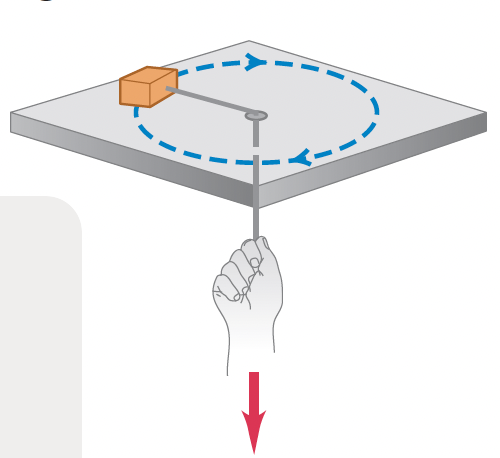
\includegraphics[width=0.5\linewidth]{../figures/P6_71.png}
  \label{fig:P6_71}
\end{figure}

A small block with a mass of \qty{0,0600}{kg} is attached to a cord passing through a hole in a frictionless, horizontal surface (\textbf{\autoref{fig:P6_71}}). The block is originally revolving at a distance of \qty{0,40}{m} from the hole with a speed of \qty{0,70}{m/s}. The cord is then pulled from below, shortening the radius of the circle in which the block revolves to \qty{0,10}{m}. At this new distance, the speed of the block is \qty{2,80}{m/s}.


\subsection*{(a)}
What is the tension in the cord in the original situation, when the block has speed $v = \qty{0,70}{\frac{m}{s}}$?
\bigbreak
For at klodsen bliver holdt i cirkelbanen kræver det at spændingen i snoren netop tilsvarer klodsens centripetalkraft. Altså har vi at
\[
T_0 = F_{c_0} = \frac{v_0^2}{R_0}m = \frac{\left( \qty{0,70}{\frac{m}{s}} \right) ^2}{\qty{0,40}{m}}\cdot \qty{0,0600}{kg} = \qty{0,0735}{N}
.\] 

\subsection*{(b)}
What is the tension in the cord in the final situation, when the block has speed $v = \qty{2,80}{\frac{m}{s}}$
\bigbreak
Med samme fremgangsmåde som ovenfor har vi at
\[
T_1 = F_{c1} = \frac{v_1^2}{R_1}m = \frac{\left( \qty{2,80}{\frac{m}{s}} \right) ^2}{\qty{0,10}{m}}\cdot \qty{0,0600}{kg} = \qty{4,70}{N}
.\] 


\subsection*{(c)}
How much work was done by the person who pulled on the cord?
\bigbreak
Arbejdet svarer til ændringen i den kinetiske energi. Altså har vi at
\[
W = \Delta k = \frac{1}{2}m\cdot \left( v_1^2-v_0^2 \right) = \frac{1}{2}\qty{0,0600}{kg} \cdot \left( \left( \qty{2,80}{\frac{m}{s}} \right)^2 - \left( \qty{0,70}{\frac{m}{s}} \right)^2 \right) = \qty{0,2205}{J}
.\] 

\section*{Opg. 6.76}
The spring of a spring gun has force constant $k = \qty{400}{\frac{N}{m}}$ and negligible mass. The spring is compressed \qty{6,00}{cm}, and a ball with mass \qty{0,0300}{kg} is placed in the horizontal barrel against the compressed spring. The spring is then released, and the ball is propelled out the barrel of the gun. The barrel is \qty{6,00}{cm} long, so the ball leaves the barrel at the same point that it loses contact with the spring. The gun is held so that the barrel is horizontal.


\subsection*{(a)}
Calculate the speed with which the ball leaves the barrel if you can ignore friction.
\bigbreak
Idet det antages at der ikke er nogen friktion må alt den potentielle energi i fjederen blive omdannet til kinetisk energi. Altså har vi at
\[
k = U_{el} = \frac{1}{2}kx^2 = \frac{1}{2}\cdot \qty{400}{\frac{N}{m}}\cdot \left( \qty{6,00}{cm} \right)^2 = \qty{0,72}{J}
.\] 
For at kuglen kan have en kinetisk energi på \qty{0,72}{J} må dens hastighed være
\[
v = \sqrt{\frac{2k}{m}} = \sqrt{\frac{2\cdot \qty{0,72}{J}}{\qty{0,0300}{kg}}} = \qty{6,93}{\frac{m}{s}}  
.\] 

\subsection*{(b)}
Calculate the speed of the ball as it leaves the barrel if a constant resisting force of \qty{6,00}{N} acts on the ball as it moves along the barrel.
\bigbreak
Det samlede arbejde må være summen af arbejdet på kuglen fra opgaven før og arbejdet af friktionskraften. Altså har vi at
\[
W_{tot} = k - \qty{6,00}{N}\cdot \qty{6,00}{cm} = \qty{0,36}{J}
.\] 
Og dermed
\[
v = \sqrt{\frac{2\cdot \qty{0,36}{J}}{\qty{0,0300}{kg}}} = \qty{4,90}{\frac{m}{s}}
.\] 

\subsection*{(c)}
For the situation in part \textbf{(b)}, at what position along the barrel does the ball have the greatest speed, and what is that speed? (In this case, the maximum speed does not occur at the end of the barrel.)
\bigbreak
Kuglen må have den største hastighed netop i det punkt, hvor dens acceleration er 0. Dette punkt må ligeledes være det punkt for den samlede kraft er 0. Altså har vi at:
\[
F_{tot} = F_s - F_\mu = kx - F_\mu = 0
.\] 
Hvilket kan omskrives til
\[
k\Vec{x} = F_\mu \implies \Vec{x} = \frac{F_\mu}{k} = \frac{\qty{6,00}{N}}{\qty{400}{\frac{N}{m}}} = \qty{1,5}{cm}
.\] 
Altså er hastigheden størst når fjederen er trykket sammen med \qty{1,5}{cm}, dvs. når kuglen er \qty{1,5}{cm} fra spidsen af pistolen. Det samlede arbejde udført på dette tidspunkt er givet ved
\[
W_{tot} = W_s - W_\mu = \frac{1}{2}\cdot \qty{400}{\frac{N}{m}} \cdot \left( \left( \qty{6,0}{cm} \right)^2 - \left( \qty{1,5}{cm} \right)^2  \right) - \qty{6,00}{N}\cdot \qty{4,5}{cm} = \qty{0,405}{J}
.\] 
Hastigheden af kuglen på dette tidspunkt er derfor
\[
v = \sqrt{\frac{2\cdot \qty{0,405}{J}}{\qty{0,0300}{kg}}} = \qty{5,20}{\frac{m}{s}}
.\] 



\section*{Opg. 6.81}

\begin{figure} [ht]
  \centering
  \caption{}
  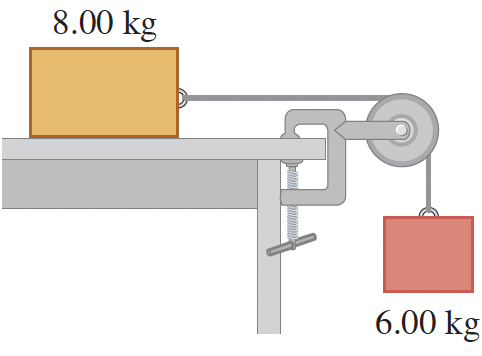
\includegraphics[width=0.5\linewidth]{../figures/P6_81.png}
  \label{fig:P6_81}
\end{figure}

Consider the system shown in (\textbf{\autoref{fig:P6_81}}). The rope and pulley have negligible mass, and the pulley is frictionless. Initially the \qty{6,00}{kg} block is moving downward and the \qty{8,00}{kg} block is moving to the right, both with a speed of \qty{0,900}{m/s}. The blocks come to rest after moving \qty{2,00}{m}. Use the work–energy theorem to calculate the coefficient of kinetic friction between the \qty{8,00}{kg} block and the tabletop.
\bigbreak
Fra "the work-energy theorem" har vi at det totale arbejde netop må tilsvare ændringen i kinetisk energi. Altså har vi at
\[
\Delta k = \left( F_t - F_\mu \right) \Delta s \implies \frac{1}{2} (m_1+m_2) \left( 0 - v_1^2 \right)  = \left( m_2 \cdot g - N_1 \cdot \mu \right)\Delta x  
.\]
Gnidningskoefficienten kan dernæst isoleres:
\begin{align*}
  m_2\cdot g - m_1\cdot g\cdot \mu &= - \frac{(m_1 + m_2)\cdot v_1^2}{2\Delta x} \\
  m_1\cdot g\cdot \mu &= \frac{(m_1 + m_2)\cdot v_1^2}{2\Delta x} + m_2\cdot g \\
  \mu &= \frac{(m_1 + m_2) \cdot v_1^2}{2\Delta x \cdot m_1 g} + \frac{m_2}{m_1}
.\end{align*}
Og altså får vi at
\[
  \mu = \frac{\left( \qty{8,00}{kg} + \qty{6,00}{kg} \right) \cdot \left(\qty{0,900}{\frac{m}{s}}\right)^2}{2\cdot \qty{2,00}{m}\cdot \qty{8,00}{kg}\cdot \qty{9,81}{\frac{m}{s^2}}} + \frac{\qty{6,00}{kg}}{\qty{8,00}{kg}} =  0,786
.\]


\end{document}
